\chapter{Introduction}
\label{chap:prod:introduction}

The measurement of cross-sections is one of the most fundamental measurements a 
particle physics experiment can make.
This \namecref{chap:prod} describes a measurement of charm and \ccbar\ 
production, performed using the \lhcb\ detector with data taken at $\sqrts = 
\SI{13}{\TeV}$.
At the \ac{LHC}, a given charm hadron \PHc\ can either be produced in the 
proton-proton interaction, directly or in the strong decay of some excited 
charm state, or in the decays of \PB hadrons.
The latter mechanism is called \emph{secondary} production, whilst the former is called \emph{prompt} production.
The type of charm hadron that can be produced can either be \emph{charmonium}, such as the \PJpsi meson, which contains charm quarks but whose net charm quantum number is zero, or \emph{open charm}, whose net charm quantum number is non-zero.
This measurement is concerned with the prompt production of open charm hadrons.
No attempt is made to distinguish between the two types of prompt production.

Measurements of \ccbar\ and \bbbar\ cross-sections at the \ac{LHC} are made to 
test the predictions of \acf{QCD}.
The production rate of heavy flavour hadrons is expected to vary as a function 
of hadron \pT\ and rapidity \rapidity, defined as
\begin{equation}
  y = \frac{1}{2}\ln{\frac{E + p_{z}}{E - p_{z}}},
  \label{eqn:prod:introduction:rapidity}
\end{equation}
and so experimental measurements can be compared with both the shape of 
theoretical predictions as a function of \pTy, as well as to the total 
integrated rate.
They can also be used as inputs to constrain future predictions.
Heavy flavour production rates are also used to estimate sensitivities for experimental searches 
for rare decays, and also as inputs to 
atmospheric neutrino experiments, where charm production enters as a background 
process.

Measuring \ccbar\ and \bbbar\ cross-sections at \lhcb\ is complementary to such 
measurements by the \acp{GPD}, due to the unique rapidity range it instruments, 
as well as its ability to cleanly reconstruct low \pT\ hadrons.

\section{Analysis overview}
\label{chap:prod:introduction:analysis_overview}

The cross-section for the inclusive production of an open charm hadron \PHc\ 
from proton-proton collisions can be expressed by rearranging 
\cref{eqn:intro:lhc:lumi_xsec}
\begin{equation}
  \xsec(\ppToHc{}X) = \frac{N(\PHc)}{\intlumi},
  \label{eqn:prod:introduction:simple_cross_section}
\end{equation}
where $N(\PHc)$ is the total number of \PHc\ hadrons that were produced, and 
\intlumi\ is the instantaneous luminosity \emph{integrated} over the time 
corresponding to the dataset used to measure $N(\PHc)$
\begin{equation}
  \intlumi = \int \lumi \dif{t}.
  \label{eqn:prod:introduction:integrated_lumi}
\end{equation}
Experimentally, not all hadrons that are produced are observed, firstly due to 
the inefficiency of the detector and the reconstruction and selection criteria, 
and secondly due to the hadrons being reconstructed in a specific final state 
$f$, to which the hadron will only decay with a particular probability.
The \emph{measured} yield $N(\HcTof)$ is then corrected for these factors, and the 
cross-section is defined as
\begin{equation}
  \xsec(\PHc) = \frac{%
    N(\HcTof)
  }{%
    \eff(\HcTof)\cdot\bfrac(\HcTof)\cdot\intlumi
  },
  \label{eqn:prod:introduction:cross_section}
\end{equation}
where \eff\ is the efficiency of fully reconstructing and selecting the decay 
\HcTof, given that it was produced, \bfrac\ is the branching fraction of the 
decay, and the inclusive production from proton-proton collisions is now 
implicit.
To compare with the shapes of theoretical predictions, double differential 
cross-sections can be determined in bins of charm hadron \pT\ and \rapidity, 
using the width $\Delta\pT$ of the bin in \pT\ and the width $\Delta\rapidity$ 
of the bin in rapidity in which the yield and efficiency measurements were made
\begin{equation}
  % There is a "\left." here, which is invisible, to balance the "\right\rvert"
  \left.\frac{\dif^{2}{\xsec(\PHc)}}{\dif{\pT}\dif{\rapidity}}\right\rvert_{i}
    = \frac{1}{\Delta\pT\Delta\rapidity}
      \frac{%
        N_{i}(\HcTof)
      }{%
        \eff_{i}(\HcTof)\cdot\bfrac(\HcTof)\cdot\intlumi
      },
  \label{eqn:prod:introduction:differential_cross_section}
\end{equation}
where the $i$ is the index of the \pTy\ bin in which the measurement is made.
The branching fraction and the integrated luminosity are the same across all bins.

This analysis measures the double differential cross-sections of \PDzero, \PDp, 
\PDsplus, and \PDstarp open charm mesons.\footnotemark
The final states chosen are \DzToKpi, \DpToKpipi, \DspTophipi with \phiToKK, 
and \DstToDzpi with \DzToKpi, the branching fractions of which are listed in 
\cref{tab:prod:introduction:branching_ratios}.
Charge conjugation is implied, in that the cross-sections measure the combined 
rate of meson and anti-meson production.
The measurements are made in the \pT\ range $0 < \pT < \SI{15}{\GeVc}$ and the 
rapidity range $2 < \rapidity < 4.5$.
In \rapidity, the measurements are made in five bins of width 0.5, and in \pT\ 
the bins are \SI{1}{\GeVc} in width in the regions $0 < \pT < \SI{1}{\GeVc}$ 
and $4 < \pT < \SI{15}{\GeVc}$, and are \SI{0.5}{\GeVc} in width in the region 
$1 < \pT < \SI{4}{\GeVc}$.

\footnotetext{%
  The excited \PD state is, formally, the \PDstp\ meson, but will be referred 
  to throughout as `\PDstarp'.
}

\begin{table}
  \centering
  \caption{%
      Branching ratios for the different decay 
      modes~\cite{PDG2014,Alexander:2008aa}.
  }
  \label{tab:prod:introduction:branching_ratios}
  \begin{tabular}{lS[table-format=1.2(2)]}
  \toprule
  Decay mode  & {\bfrac\ (\si{\percent})} \\
  \midrule
  \DzToKpi    & 3.88 \pm 0.05             \\
  \DpToKpipi  & 9.13 \pm 0.19             \\
  \DspTophipi & 2.24 \pm 0.13             \\
  \DstToDzpi  & 67.7 \pm 0.5              \\
  \bottomrule
\end{tabular}

\end{table}

From the double differential measurements, several derived quantities are 
computed, namely the ratio of charm production rates measured at $\sqrts = 
\SI{13}{\TeV}$ and those measured by \lhcb\ at 
\SI{7}{\TeV}~\cite{LHCb-PAPER-2012-041}, ratios of production rates between 
charm mesons, open charm hadron cross-sections integrated across the \pTy\ 
space, and integrated \ccbar\ cross-sections.
Each integrated per-meson cross-section is the sum over all \pTy\ bins of the 
respective double differential measurements
\begin{equation}
  \xsec{(\PHc)} =
    \sum_{i}^{N} \xsec_{i}(\PHc).
  \label{eqn:prod:introduction:integrated_cross_section}
\end{equation}
The total \ccbar\ cross-sections can be computed using \emph{fragmentation 
  fractions}; each a measurement of the transition probability that a charm 
quark will hadronise to a particular open charm hadron $f(\cToHc)$.
Given the fragmentation fraction, and the integrated cross-section defined in 
\cref{eqn:prod:introduction:integrated_cross_section}, the integrated \ccbar\ 
cross-section can be computed as
\begin{equation}
  \xsec{(\ccbar)} = \frac{\xsec(\PHc + \APHc)}{2f(\cToHc)}.
  \label{eqn:prod:introduction:ccbar_cross_section}
\end{equation}
The factor $\sfrac{1}{2}$ arises from the fragmentation fraction not accounting 
for charge conjugate (anti-charm) states, which have been noted explicitly here 
in the expression for the measured cross-section to avoid ambiguity.
For this analysis, the fragmentation fractions are taken from the 
\ac{PDG}~\cite{PDG2008}, who compute them as averages of measurements made at 
\epem\ colliders operating at a centre-of-mass energy close to the 
\PUpsilonFourS resonance.
These values are given in \cref{tab:prod:introduction:fragmentation_fractions}, 
where the transition probability for \PDzero, $f(\decay{\Pcharm}{\PDzero})$, 
includes contributions from \DstToDzpi\ decays.

\begin{table}
  \caption[Charm hadron fragmentation fractions]{%
    Charm hadron fragmentation fractions~\cite{PDG2008}.
    Here, \PHc\ does not include the charge conjugate state.
  }
  \label{tab:prod:introduction:fragmentation_fractions}
  \centering
  \begin{tabular}{cc}
  \toprule
  $\PHc$   & $f(\cToHc)$       \\
  \midrule
  \PDz     & $0.565 \pm 0.032$ \\
  \PDp     & $0.246 \pm 0.020$ \\
  \PDsplus & $0.224 \pm 0.028$ \\
  \PDstarp & $0.080 \pm 0.017$ \\
  \bottomrule
\end{tabular}

\end{table}

\subsection{Treatment of uncertainties}
\label{chap:prod:introduction:uncertainties}

Throughout this analysis, the method of \acl{MC} error propagation is used.
With this, each quantity entering 
\cref{eqn:prod:introduction:differential_cross_section} is assumed to be drawn 
from some \acf{PDF} with a known set of parameters, and then ten thousand 
numbers are sampled from that \ac{PDF}.
When performing operations using such quantities, the operations are performed 
on the input sample vectors, and then statistics on the result can be computed 
on the new, resulting sample vector.
This technique is used as error analysis of the measurement is complex: what 
enters into the cross-section is the inverse of the efficiency, for example, 
the corresponding \acl{PDF} of which may be obvious, in particular whether the 
uncertainties can be treated as Gaussian.
The use of \ac{MC} error propagation simplifies such analysis.

An example cross-section, measured in the region \pTyrange{12}{13}{2.5}{3}, is 
given in \cref{fig::prod:introduction:uncertainties:posterior}.
The blue curve shows the \ac{PDF} of the cross-section when only the 
statistical uncertainty is considered, whilst the green curve also includes the 
contributions from the systematic uncertainties.
The green curve is not symmetric, and the mode is shifted with respect to the 
blue.

Unless stated otherwise, each quantity that is measured directly is assumed to 
follow a normal distribution, whose mean is equal to the measured value, and 
whose width is equal to the measured uncertainty on that value.
The computation of that measured uncertainty will be described when the 
respective measurements are presented.
When the result of operations using such measurements is presented, such as 
cross-sections, the central value given is the most probable value of the 
sample vector representing the result, and the lower and upper uncertainty 
bounds are given by the \SI{15.9}{\percent} and \SI{84.1}{\percent} percentiles 
either side of the central value.

\begin{figure}
  \centering
  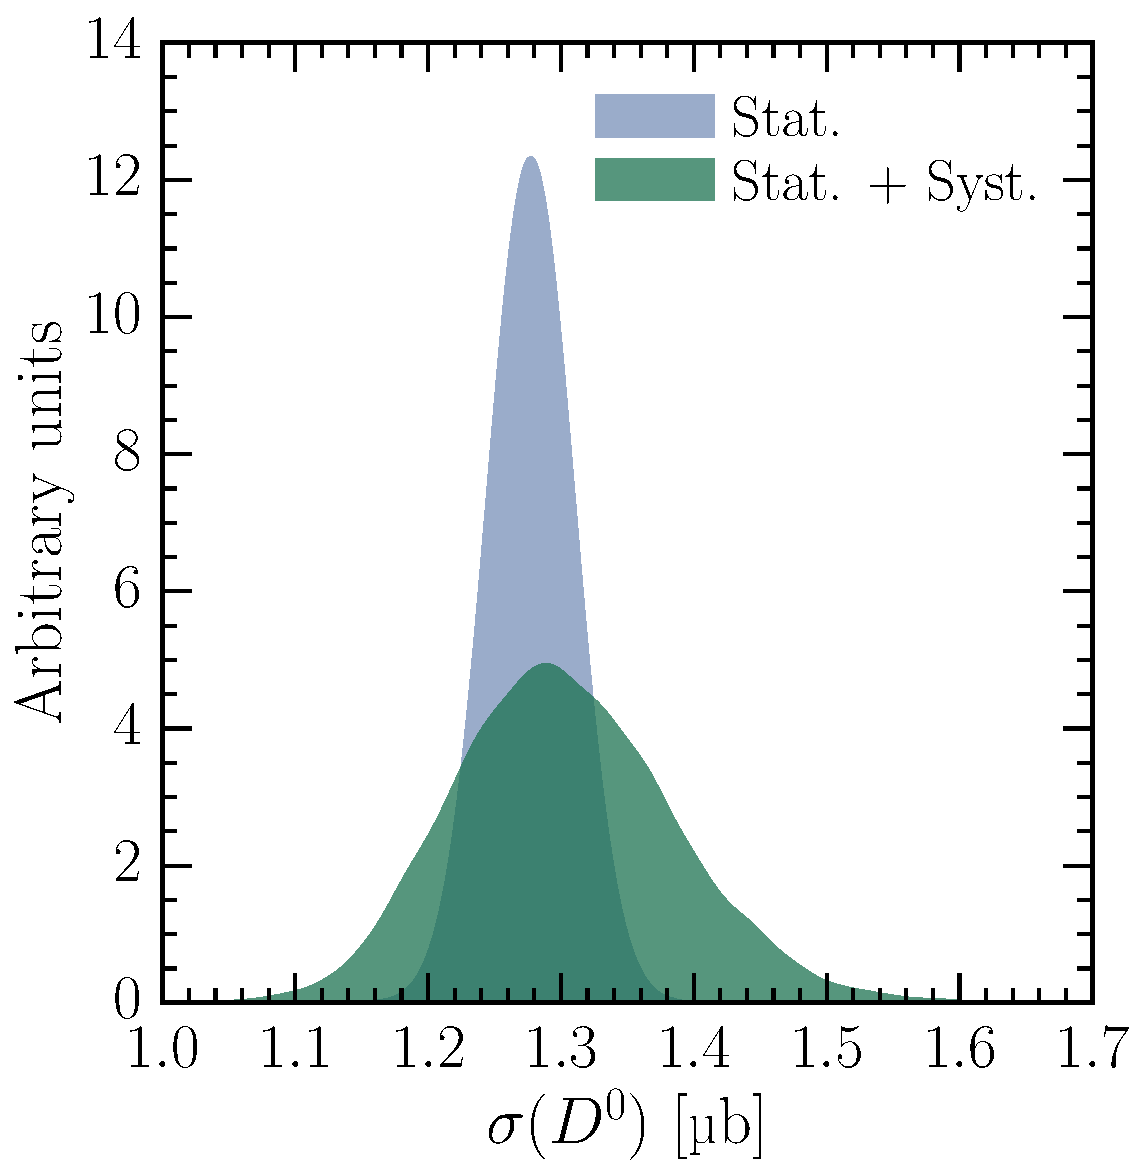
\includegraphics[width=\linewidth]{production/D0ToKpi_posterior_pdf}
  \caption{%
    Posterior probability densities for a measurement of the \PDzero 
    cross-section in the region \pTyrange{12}{13}{2.5}{3}.
    The blue curve shows the density including contributions only from the 
    statistical uncertainty on the prompt signal count.
    The green curve shows the density including contributions from all 
    uncertainties that enter the measurement.
  }
  \label{fig::prod:introduction:uncertainties:posterior}
\end{figure}

\subsection{Document structure}
\label{chap:prod:introduction:structure}

The data used for the measurements were collected in July 2016, under a set of 
special conditions used for the restart of the \ac{LHC} after \ac{LS1}.
The conditions of the \ac{LHC} and of the \lhcb\ detector will be described in 
\cref{chap:prod:data}, along with a description of the corresponding simulated 
data and a summary of the integrated luminosity measurement.
After collection, the data are reconstructed and selected to build charm hadron 
candidates, which will be presented in \cref{chap:prod:sel}.
The extraction of the prompt yields is made on the fully reconstructed and 
selected data using the method of maximum likelihood fits, as described in 
\cref{chap:prod:fitting}.
The evaluation of the associated efficiencies is performed using a mixture of 
simulated \acl{MC} data and dedicated calibration samples, and is discussed in 
\cref{chap:prod:effs}, after which the systematic uncertainties associated with 
all procedures used in the measurement are evaluated, for which the description 
and results are given in \cref{chap:prod:syst}.
Finally, the cross-sections themselves are computed, and are presented in 
\cref{chap:prod:results}.

Before the discussion on the experimental methods and the results, further 
motivation for performing measurements heavy flavour cross-sections, both 
theoretical and experimental, will be presented in the following 
\namecref{chap:prod:theory}.
